\documentclass[11pt]{article}

\usepackage{amsmath}
\usepackage{amsfonts}
\usepackage{amsthm}
\usepackage{blkarray}
\usepackage{caption}
\usepackage{enumitem}
\usepackage{graphicx}
\usepackage{hyperref}
\usepackage{mathtools}
\usepackage{tikz}
\usepackage[top=1.5cm,bottom=2cm,left=1.25cm,right=1.75cm,marginparwidth=1.75cm]{geometry}
\setlength{\parindent}{0cm}

\newcommand{\R}{\mathbb{R}}
\newcommand{\n}{\vspace{0.3cm}}
\newtheorem{theorem}{Theorem}

\def\lc{\left\lceil}
\def\rc{\right\rceil}
\def\lf{\left\lfloor}
\def\rf{\right\rfloor}

\title{\vspace{-1.0cm}CSCI 5304 Homework 2 }
\author{Fletcher Gornick}
\date{October 5}

\begin{document}
\maketitle
\begin{enumerate}
	\item \begin{enumerate}
		      \item Solve the linear system \(Ax = b\) by Gaussian elimination, where:
		            \[A =
			            \begin{pmatrix*}[r]
				            1  & -2 & -1 & 0  \\
				            -2 & 3  & 2  & 1  \\
				            -1 & 2  & 3  & -2 \\
				            0  & -1 & -4 & 6
			            \end{pmatrix*}
			            \quad b = \begin{pmatrix*}[r] -3 \\ 5 \\ 1 \\ 4 \end{pmatrix*}
		            \]
		            We proceed by performing a series of row operations, keeping track of the corresponding elementary matrices \(M_1\), \(M_2\), and \(M_3\).
		            \begin{align*}
			            M_1 (A \mid b)         & =
			            \begin{pmatrix*}[r]
				            1 & 0 & 0 & 0 \\
				            2 & 1 & 0 & 0 \\
				            1 & 0 & 1 & 0 \\
				            0 & 0 & 0 & 1
			            \end{pmatrix*}
			            \left(\begin{array}{rrrr|r}
					                  1  & -2 & -1 & 0  & -3 \\
					                  -2 & 3  & 2  & 1  & 5  \\
					                  -1 & 2  & 3  & -2 & 1  \\
					                  0  & -1 & -4 & 6  & 4
				                  \end{array}\right)
			                                   & =
			            \left(\begin{array}{rrrr|r}
					                  1 & -2 & -1 & 0  & -3 \\
					                  0 & -1 & 0  & 1  & -1 \\
					                  0 & 0  & 2  & -2 & -2 \\
					                  0 & -1 & -4 & 6  & 4  \\
				                  \end{array}\right)                                \\
			            M_2 M_1 (A \mid b)     & =
			            \begin{pmatrix*}[r]
				            1 & 0  & 0 & 0 \\
				            0 & 1  & 0 & 0 \\
				            0 & 0  & 1 & 0 \\
				            0 & -1 & 0 & 1 \\
			            \end{pmatrix*}
			            \left(\begin{array}{rrrr|r}
					                  1 & -2 & -1 & 0  & -3 \\
					                  0 & -1 & 0  & 1  & -1 \\
					                  0 & 0  & 2  & -2 & -2 \\
					                  0 & -1 & -4 & 6  & 4
				                  \end{array}\right)
			                                   & =
			            \left(\begin{array}{rrrr|r}
					                  1 & -2 & -1 & 0  & -3 \\
					                  0 & -1 & 0  & 1  & -1 \\
					                  0 & 0  & 2  & -2 & -2 \\
					                  0 & 0  & -4 & 5  & 5  \\
				                  \end{array}\right)                                \\
			            M_3 M_2 M_1 (A \mid b) & =
			            \begin{pmatrix*}[r]
				            1 & 0 & 0 & 0 \\
				            0 & 1 & 0 & 0 \\
				            0 & 0 & 1 & 0 \\
				            0 & 0 & 2 & 1 \\
			            \end{pmatrix*}
			            \left(\begin{array}{rrrr|r}
					                  1 & -2 & -1 & 0  & -3 \\
					                  0 & -1 & 0  & 1  & -1 \\
					                  0 & 0  & 2  & -2 & -2 \\
					                  0 & 0  & -4 & 5  & 5  \\
				                  \end{array}\right)
			                                   & =
			            \left(\begin{array}{rrrr|r}
					                  1 & -2 & -1 & 0  & -3 \\
					                  0 & -1 & 0  & 1  & -1 \\
					                  0 & 0  & 2  & -2 & -2 \\
					                  0 & 0  & 0  & 1  & 1  \\
				                  \end{array}\right)                                \\
			                                   & = L^{-1}(A \mid b) = (U \mid L b)
		            \end{align*}
		            Now we have an augmented upper-triangular matrix with one solution.  We can back-solve from here to get all values of \(x\).
		            \begin{align*}
			            x_4                                                          & = 1 \\
			            2x_3 - 2x_4 = -2 \implies 2x_3 - 2 = -2 \implies x_3         & = 0 \\
			            -x_2 + x_4 = -1 \implies -x_2 + 1 = -1 \implies x_2          & = 2 \\
			            x_1 - 2x_2 - x_3 = -3 \implies x_1 - 4 - 0 = -3 \implies x_1 & = 1
		            \end{align*}
		            This tells us \(x = (1,2,0,1)^T\). \n

		      \item What is the LU factorization of \(A\), what is it's determinant? \n\\
		            \(U\) and \(L^{-1}\) were derived in (a), and retrieving \(L\) from \(L^{-1}\) is as simple as negating the elements below the diagonal, so we get:
		            \[
			            L = (M_3 M_2 M_1)^{-1}
			            =
			            \begin{pmatrix*}[r]
				            1 & 0  & 0 & 0 \\
				            2 & 1  & 0 & 0 \\
				            1 & 0  & 1 & 0 \\
				            0 & -1 & 2 & 1
			            \end{pmatrix*}^{-1}
			            =
			            \begin{pmatrix*}[r]
				            1  & 0 & 0  & 0 \\
				            -2 & 1 & 0  & 0 \\
				            -1 & 0 & 1  & 0 \\
				            0  & 1 & -2 & 1
			            \end{pmatrix*}, \;\;
			            U =
			            \begin{pmatrix*}[r]
				            1 & -2 & -1 & 0  \\
				            0 & -1 & 0  & 1  \\
				            0 & 0  & 2  & -2 \\
				            0 & 0  & 0  & 1
			            \end{pmatrix*}
		            \]
		            Now, since \(A = LU\), we know \(\det(A) = \det(L)\det(U)\), making \[\det(A) = (1 \cdot 1 \cdot 1 \cdot 1) \cdot (1 \cdot (-1) \cdot 2 \cdot 1) = -2.\]

		      \item Using the LU factors obtained in (b), find the last column of the inverse of \(A\), without computing the whole inverse. \n\\
		            First note that \((L^{-1})_{:,n} = e_n\), so the only nonzero value of \((L^{-1})_{:,n}\) is \((L^{-1})_{n,n} = 1\),
		            \[(A^{-1})_{:,n} = \sum_{k=1}^n (U^{-1})_{:,k}(L^{-1})_{k,n} = (U^{-1})_{:,n}\]
		            Since \(U\) is upper-triangular, finding the \((U^{-1})_{:,n}\) can be done relatively quickly:
		            \begin{align*}
			            (U \mid I) & = \left(\begin{array}{rrrr|rrrr}
					                                 1 & -2 & -1 & 0  & 1 & 0 & 0 & 0 \\
					                                 0 & -1 & 0  & 1  & 0 & 1 & 0 & 0 \\
					                                 0 & 0  & 2  & -2 & 0 & 0 & 1 & 0 \\
					                                 0 & 0  & 0  & 1  & 0 & 0 & 0 & 1 \\
				                                 \end{array}\right)
			                       & \to                                 &
			            \left(\begin{array}{rrrr|rrrr}
					                  1 & -2 & -1 & 0  & 1 & 0  & 0       & 0 \\
					                  0 & 1  & 0  & -1 & 0 & -1 & 0       & 0 \\
					                  0 & 0  & 1  & -1 & 0 & 0  & \frac12 & 0 \\
					                  0 & 0  & 0  & 1  & 0 & 0  & 0       & 1 \\
				                  \end{array}\right)         \\
			                       & \to
			            \left(\begin{array}{rrrr|rrrr}
					                  1 & -2 & -1 & 0 & 1 & 0  & 0       & 0 \\
					                  0 & 1  & 0  & 0 & 0 & -1 & 0       & 1 \\
					                  0 & 0  & 1  & 0 & 0 & 0  & \frac12 & 1 \\
					                  0 & 0  & 0  & 1 & 0 & 0  & 0       & 1 \\
				                  \end{array}\right)
			                       & \to                                 &
			            \left(\begin{array}{rrrr|rrrr}
					                  1 & -2 & 0 & 0 & 1 & 0  & \frac12 & 1 \\
					                  0 & 1  & 0 & 0 & 0 & -1 & 0       & 1 \\
					                  0 & 0  & 1 & 0 & 0 & 0  & \frac12 & 1 \\
					                  0 & 0  & 0 & 1 & 0 & 0  & 0       & 1 \\
				                  \end{array}\right)           \\
			                       & \to
			            \left(\begin{array}{rrrr|rrrr}
					                  1 & 0 & 0 & 0 & 1 & -2 & \frac12 & 3 \\
					                  0 & 1 & 0 & 0 & 0 & -1 & 0       & 1 \\
					                  0 & 0 & 1 & 0 & 0 & 0  & \frac12 & 1 \\
					                  0 & 0 & 0 & 1 & 0 & 0  & 0       & 1 \\
				                  \end{array}\right)
			                       & \to                                 &
			            \;\;U^{-1} =
			            \begin{pmatrix*}[r]
				            1 & -2 & \frac12 & 3 \\
				            0 & -1 & 0   & 1 \\
				            0 & 0  & \frac12 & 1 \\
				            0 & 0  & 0   & 1 \\
			            \end{pmatrix*}
		            \end{align*}
		            So we can see that \((A^{-1})_{:,4} = (U^{-1})_{:,4} = (3,1,1,1)^T\).
	      \end{enumerate}

	\item Let \(A = LU\) be the LU factorization of \(A \in \R^{n \times n}\), with \(|\ell_{i,j}| \leq 1\).  Verify the equation:
	      \[u_{i,:} = a_{i,:} - \sum_{j=1}^{i-1} \ell_{i,j}u_{j,:},\]
	      Then use this relation to show that \(\lVert U \rVert_\infty \leq 2^{n-1} \lVert A \rVert_\infty\).

	      \begin{proof}
		      First, we can acquire this equation for \(a_{i,:}\) by noting that \(\ell_{i,j} = 0\) for all \(j>i\):
		      \[a_{i,:} = (\ell u)_{i,:} = \sum_{j=1}^n \ell_{i,j}u_{j,:} = \sum_{j=1}^i \ell_{i,j}u_{j,:},\]
		      plugging this into the right-hand side of the equality we wish to prove, we see
		      \[a_{i,:} - \sum_{j=1}^{i-1} \ell_{i,j}u_{j,:} = \sum_{j=1}^i \ell_{i,j}u_{j,:} - \sum_{j=1}^{i-1} \ell_{i,j}u_{j,:} = \ell_{i,i}u_{i,:} = 1 \cdot u_{i,:} = u_{i,:}.\]


		      To show \(\lVert U \rVert_\infty \leq 2^{n-1}\lVert A \rVert_\infty\) we proceed inductively.

		      Let \(i_0\) be the index of the the maximum row of \(U\), that is, \(\lVert U \rVert_\infty = \max_i \lVert u_{i,:} \rVert_1 = \lVert u_{i_0,:} \rVert_1\).  If \(i_0 = 1\), then clearly \(\lVert U \rVert_\infty = \lVert u_{1,:} \rVert_1 = \lVert a_{1,:} \rVert_1 \leq \lVert A \rVert_\infty \leq 2^{n-1}\lVert A \rVert_\infty\).

		      Now, suppose for all \(k \geq 2\), \(\lVert u_{k,:} \rVert_1 \leq 2^{k-1}\lVert A \rVert_\infty\), we show \(\lVert u_{k+1,:} \rVert_1 \leq 2^k \lVert A \rVert_\infty.\)

		      \begin{align*}
			      \lVert u_{k+1,:} \rVert_1 & = \left\lVert a_{k+1,:} - \sum_{j=1}^k \ell_{k+1,j} u_{j,:} \right\rVert_1                                              & (\text{derived above})                             \\
			                                & \leq \lVert a_{k+1,:} \rVert_1 + \sum_{j=1}^k \lVert u_{j,:} \rVert_1                                                   & (\text{triangle inequality})                       \\
			                                & \leq \lVert A \rVert_\infty + \lVert u_{1,:} \rVert_1 + \lVert u_{2,:} \rVert_1 + \dots + \lVert u_{k,:} \rVert_1       & (\text{definition of } \lVert \cdot \rVert_\infty) \\
			                                & \leq \lVert A \rVert_\infty + \lVert A \rVert_\infty + 2\lVert A \rVert_\infty + \dots + 2^{k-1}\lVert A  \rVert_\infty & (\text{inductive hypothesis})                      \\
			                                & = 2\lVert A \rVert_\infty + 2\lVert A \rVert_\infty + \dots + 2^{k-1}\lVert A \rVert_\infty                             & (\text{merge first 2 terms})                       \\
			                                & = 2\lVert A \rVert_\infty \left( 1 + 1 + 2 + 4 + \dots + 2^{k-2}\right)                                                 & (\text{pull out } 2 \lVert A \rVert_\infty)        \\
			                                & = 2 \cdot 2^{k-1} \lVert A \rVert_\infty                                                                                & (\text{obvious in binary})                         \\
			                                & = 2^k \lVert A \rVert_\infty.                                                                                           &
		      \end{align*}
		      Since \(\lVert u_{i,:} \rVert_1 \leq 2^{i-1} \lVert A \rVert_\infty\) for all rows \(i\), and the largest possible value for \(i\) is \(n\), we can conclude \(\lVert U \rVert_\infty \leq 2^{n-1}\lVert A \rVert_\infty\) by the principle of strong mathematical induction.
	      \end{proof}


	\item For the following matrix:
	      \[A =
		      \begin{pmatrix*}[r]
			      1 & -1 & 1 \\
			      0 & 4  & 2 \\
			      6 & 2  & 0
		      \end{pmatrix*}
	      \]
	      \begin{enumerate}
		      \item Determine the standard LU factorization of the matrix.
		            \begin{align*}
			            M_1 A                & =
			            \begin{pmatrix*}[r]
				            1  & 0 & 0 \\
				            0  & 1 & 0 \\
				            -6 & 0 & 1
			            \end{pmatrix*}
			            \begin{pmatrix*}[r]
				            1 & -1 & 1 \\
				            0 & 4  & 2 \\
				            6 & 2  & 0
			            \end{pmatrix*}
			                                 & = &
			            \begin{pmatrix*}[r]
				            1 & -1 & 1  \\
				            0 & 4  & 2  \\
				            0 & 8  & -6
			            \end{pmatrix*}         \\
			            L^{-1} A = M_2 M_1 A & =
			            \begin{pmatrix*}[r]
				            1 & 0  & 0 \\
				            0 & 1  & 0 \\
				            0 & -2 & 1
			            \end{pmatrix*}
			            \begin{pmatrix*}[r]
				            1  & 0 & 0 \\
				            0  & 1 & 0 \\
				            -6 & 0 & 1
			            \end{pmatrix*}
			            \begin{pmatrix*}[r]
				            1 & -1 & 1 \\
				            0 & 4  & 2 \\
				            6 & 2  & 0
			            \end{pmatrix*}
			                                 & = &
			            \begin{pmatrix*}[r]
				            1 & -1 & 1   \\
				            0 & 4  & 2   \\
				            0 & 0  & -10
			            \end{pmatrix*}
			            = U
		            \end{align*}

		            \[
			            L =
			            \begin{pmatrix*}[r]
				            1  & 0  & 0 \\
				            0  & 1  & 0 \\
				            -6 & -2 & 1
			            \end{pmatrix*}^{-1}
			            =
			            \begin{pmatrix*}[r]
				            1 & 0 & 0 \\
				            0 & 1 & 0 \\
				            6 & 2 & 1
			            \end{pmatrix*}, \;\;
			            U =
			            \begin{pmatrix*}[r]
				            1 & -1 & 1   \\
				            0 & 4  & 2   \\
				            0 & 0  & -10
			            \end{pmatrix*}.
		            \]

		      \item Compute the determinant of \(A\).
		            \[\det(A) \;=\; \det(L)\det(U) \;=\; (1 \cdot 1 \cdot 1) \cdot (1 \cdot 4 \cdot -10) \;=\; -40.\]

		      \item Compute the first column of the inverse of \(A\)
		            \begin{align*}
			            \left(\begin{array}{rrr|rrr}
					                  1 & -1 & 1   & 1 & 0 & 0 \\
					                  0 & 4  & 2   & 0 & 1 & 0 \\
					                  0 & 0  & -10 & 0 & 0 & 1 \\
				                  \end{array}\right)
			             & \to
			            \left(\begin{array}{rrr|rrr}
					                  1 & -1 & 1       & 1 & 0       & 0             \\
					                  0 & 1  & \frac12 & 0 & \frac14 & 0             \\
					                  0 & 0  & 1       & 0 & 0       & \frac{-1}{10} \\
				                  \end{array}\right)
			             & \to &
			            \left(\begin{array}{rrr|rrr}
					                  1 & -1 & 0 & 1 & 0       & \frac{1}{10}  \\
					                  0 & 1  & 0 & 0 & \frac14 & \frac{1}{20}  \\
					                  0 & 0  & 1 & 0 & 0       & \frac{-1}{10} \\
				                  \end{array}\right) \\
			             & \to
			            \left(\begin{array}{rrr|rrr}
					                  1 & 0 & 0 & 1 & \frac14 & \frac{3}{20}  \\
					                  0 & 1 & 0 & 0 & \frac14 & \frac{1}{20}  \\
					                  0 & 0 & 1 & 0 & 0       & \frac{-1}{10} \\
				                  \end{array}\right)
			             & \to & \;\; U^{-1} =
			            \left(\begin{array}{rrr}
					                  1 & \frac14 & \frac{3}{20}  \\
					                  0 & \frac14 & \frac{1}{20}  \\
					                  0 & 0       & \frac{-1}{10} \\
				                  \end{array}\right)
		            \end{align*}
		            Unlike 1(c), we must now calculate the first column of \(A^{-1}\).  Since \((L^{-1})_{:,1} = (1,0,-6)^T\), we can get \((A^{-1})_{:,1}\) by taking
		            \[(A^{-1})_{:,1} = \sum_{k=1}^3 (U^{-1})_{:,k} (L^{-1})_{k,1} =  1 \cdot (1,0,0)^T - 6 \cdot \left(\tfrac{3}{20}, \tfrac{1}{20}, \tfrac{-1}{10}\right)^T = \left(\tfrac{1}{10}, \tfrac{-3}{10}, \tfrac35\right)^T.\]


		      \item Repeat the above questions when partial pivoting is used, i.e. find the permutation matrix \(P\) and the matrices \(L,U\) such that \(PA = LU\).  Compute the determinant of \(A\) based on this factorization, and compute the first column of the inverse of \(A\), based on this factorization.

		            \begin{align*}
			            \left(\begin{array}{rrr}
					                  1 & -1 & 1 \\
					                  0 & 4  & 2 \\
					                  6 & 2  & 0 \\
				                  \end{array}\right)
			              & \to
			            \left(\begin{array}{rrr}
					                  6 & 2  & 0 \\
					                  0 & 4  & 2 \\
					                  1 & -1 & 1 \\
				                  \end{array}\right)
			            = P_{13}A
			              & \to
			            \left(\begin{array}{rrr}
					                  6 & 2          & 0 \\
					                  0 & 4          & 2 \\
					                  0 & \frac{-4}3 & 1 \\
				                  \end{array}\right)
			            = M_1 P_{13} A
			            \\
			              & \to
			            \left(\begin{array}{rrr}
					                  6 & 2 & 0       \\
					                  0 & 4 & 2       \\
					                  0 & 0 & \frac53 \\
				                  \end{array}\right)
			            = M_2 M_1 P_{13} A = U
			              & \left(
			            M_2 M_1 =
			            \left(\begin{array}{rrr}
						                  1          & 0       & 0 \\
						                  0          & 1       & 0 \\
						                  \frac{-1}6 & \frac13 & 1 \\
					                  \end{array}\right)
			            \right)                \\
			            L & = (M_2 M_1)^{-1} =
			            \left(\begin{array}{rrr}
					                  1       & 0          & 0 \\
					                  0       & 1          & 0 \\
					                  \frac16 & \frac{-1}3 & 1 \\
				                  \end{array}\right)
			              & \left(
			            P = P_{13} =
			            \left(\begin{array}{rrr}
					                  0 & 0 & 1 \\
					                  0 & 1 & 0 \\
					                  1 & 0 & 0 \\
				                  \end{array}\right)
			            \right)
		            \end{align*}
		            Now we have everything wew need to complete the decomposition.  With the matrices computed above, we get the following equality (\(PA = LU\)):
		            \[
			            \left(\begin{array}{rrr}
					            0 & 0 & 1 \\
					            0 & 1 & 0 \\
					            1 & 0 & 0 \\
				            \end{array}\right)
			            \left(\begin{array}{rrr}
					            1 & -1 & 1 \\
					            0 & 4  & 2 \\
					            6 & 2  & 0 \\
				            \end{array}\right)
			            =
			            \left(\begin{array}{rrr}
					            1       & 0          & 0 \\
					            0       & 1          & 0 \\
					            \frac16 & \frac{-1}3 & 1 \\
				            \end{array}\right)
			            \left(\begin{array}{rrr}
					            6 & 2 & 0       \\
					            0 & 4 & 2       \\
					            0 & 0 & \frac53 \\
				            \end{array}\right).
		            \]
		            To calculate the determinant, we get \(\det(PA) = \det(LU) = \det(L)\det(U) = 6 \cdot 4 \cdot \frac53 = 40\).  And since the determinant of a [odd number] row swapping elementary matrix is -1, we see that \(-1 \cdot \det(A) = 40 \implies \det(A) = -40\).

		            To compute the first column of \(A^{-1}\), we must first know \(U^{-1}\) (\(L^{-1}\) is just \(M_2 M_1\))
		            \begin{align*}
			            \left(\begin{array}{rrr|rrr}
					                  6 & 2 & 0        & 1 & 0 & 0 \\
					                  0 & 4 & 2        & 0 & 1 & 0 \\
					                  0 & 0 & \tfrac53 & 0 & 0 & 1 \\
				                  \end{array}\right)
			             & \to
			            \left(\begin{array}{rrr|rrr}
					                  1 & \tfrac13 & 0        & \tfrac16 & 0        & 0        \\
					                  0 & 1        & \tfrac12 & 0        & \tfrac14 & 0        \\
					                  0 & 0        & 1        & 0        & 0        & \tfrac35 \\
				                  \end{array}\right)
			             & \to
			            \left(\begin{array}{rrr|rrr}
					                  1 & \tfrac13 & 0 & \tfrac16 & 0        & 0              \\
					                  0 & 1        & 0 & 0        & \tfrac14 & \tfrac{-3}{10} \\
					                  0 & 0        & 1 & 0        & 0        & \tfrac35       \\
				                  \end{array}\right) \\
			             & \to
			            \left(\begin{array}{rrr|rrr}
					                  1 & 0 & 0 & \tfrac16 & \tfrac{-1}{12} & \tfrac1{10}    \\
					                  0 & 1 & 0 & 0        & \tfrac14       & \tfrac{-3}{10} \\
					                  0 & 0 & 1 & 0        & 0              & \tfrac35       \\
				                  \end{array}\right)
			             & \to
			            U^{-1} =
			            \left(\begin{array}{rrr}
					                  \tfrac16 & \tfrac{-1}{12} & \tfrac1{10}    \\
					                  0        & \tfrac14       & \tfrac{-3}{10} \\
					                  0        & 0              & \tfrac35       \\
				                  \end{array}\right)
		            \end{align*}
		            Since \((PA)^{-1} = A^{-1}P\), we know the last column of \((PA^{-1})\) is the same as the first column of \(A^{-1}\), so
		            \[A_{:,1}^{-1} = (PA)_{:,n}^{-1} = \sum_{k=1}^n (U^{-1})_{:,k}(L^{-1})_{k,n} = (U^{-1})_{:,n} = \left(\tfrac{1}{10}, \tfrac{-3}{10}, \tfrac35\right)^T.\]

	      \end{enumerate}

	\item We saw that Gaussian elimination is equivalent to multiplying the initial matrix \(A\) by a swquence of Gaussian transformations from the left.  This exercise explores what happens in the case of Gauss-Jordan (GJ) elimination.
	      \begin{enumerate}
		      \item Show that for Gauss-Jordan, we have the same result:
		            \[A_k = M_kA_{k-1}, \; k = 1, 2, \dots, n,\]
		            With \(A_0 = A\), however the matrices \(M_k\) are different.  What are the new transformations \(M_k\)?
		            \begin{proof}
			            To show this result holds for Gauss-Jordan Elimination, we must first find each matrix \(M_k\).  Let \(u_k \in \R^n\) be defined like so,
			            \[u_{ki} := \begin{cases}
					            0,                              & \text{ if } i = k, \\
					            (A_{k-1})_{ik} / (A_{k-1})_{kk} & \text{ otherwise}.
				            \end{cases}\]
			            This gives us the following definition for \(M_k\),
			            \[(M_k)_{ij} = \begin{cases}
					            1,                                & \text{ if } j = i,           \\
					            0,                                & \text{ if } j \neq i,k,      \\
					            -(A_{k-1})_{ik} / (A_{k-1})_{kk}, & \text{ if } j = k, j \neq i.
				            \end{cases}\]
			            Clearly, if \(k=1\), \(A_1 = M_1A_0\), because \(M_1\) is the same as for normal Gaussian elimination.  Now if \(A_k = M_kA_{k-1}\) for some \(k \geq 1\), we show \(A_{k+1} = M_{k+1}A_k\).
			            \footnotesize\begin{align*}
				            % M_{k+1}A_k =
				            \left(\begin{array}{cccccc}
						                  1      & 0      & \hdots & \frac{-(A_k)_{1,(k+1)}}{(A_k)_{(k+1),(k+1)}}     & \hdots & 0      \\
						                  0      & 1      & \hdots & \frac{-(A_k)_{2,(k+1)}}{(A_k)_{(k+1),(k+1)}}     & \hdots & 0      \\
						                  \vdots & \vdots & \ddots & \vdots                                           & \ddots & \vdots \\
						                  0      & 0      & \hdots & 1                                                & \hdots & 0      \\
						                  0      & 0      & \hdots & \frac{-(A_k)_{(k+2),(k+1)}}{(A_k)_{(k+1),(k+1)}} & \hdots & 0      \\
						                  \vdots & \vdots & \ddots & \vdots                                           & \ddots & \vdots \\
						                  0      & 0      & \hdots & \frac{-(A_k)_{n,(k+1)}}{(A_k)_{(k+1),(k+1)}}     & \hdots & 1      \\
					                  \end{array}\right)
				            \left(\begin{array}{ccccccc}
						                  (A_k)_{1,1} & 0           & \hdots & 0           & (A_k)_{1,(k+1)}     & \hdots & (A_k)_{1,n}     \\
						                  0           & (A_k)_{2,1} & \hdots & 0           & (A_k)_{2,(k+1)}     & \hdots & (A_k)_{2,n}     \\
						                  \vdots      & \vdots      & \ddots & \vdots      & \vdots              & \ddots & \vdots          \\
						                  0           & 0           & \hdots & (A_k)_{k,k} & (A_k)_{k,(k+1)}     & \hdots & (A_k)_{k,n}     \\
						                  0           & 0           & \hdots & 0           & (A_k)_{(k+1),(k+1)} & \hdots & (A_k)_{(k+1),n} \\
						                  \vdots      & \vdots      & \ddots & \vdots      & \vdots              & \ddots & \vdots          \\
						                  0           & 0           & \hdots & 0           & (A_k)_{n,(k+1)}     & \hdots & (A_k)_{n,n}     \\
					                  \end{array}\right)   \\
				            = \left(\begin{array}{ccccccc}
						                    (A_k)_{1,1} & 0           & \hdots & 0           & 0                   & \hdots & (A_k)_{1,n}     \\
						                    0           & (A_k)_{2,1} & \hdots & 0           & 0                   & \hdots & (A_k)_{2,n}     \\
						                    \vdots      & \vdots      & \ddots & \vdots      & \vdots              & \ddots & \vdots          \\
						                    0           & 0           & \hdots & (A_k)_{k,k} & 0                   & \hdots & (A_k)_{k,n}     \\
						                    0           & 0           & \hdots & 0           & (A_k)_{(k+1),(k+1)} & \hdots & (A_k)_{(k+1),n} \\
						                    \vdots      & \vdots      & \ddots & \vdots      & \vdots              & \ddots & \vdots          \\
						                    0           & 0           & \hdots & 0           & 0                   & \hdots & (A_k)_{n,n}     \\
					                    \end{array}\right) \\
				            = A_{k+1}
			            \end{align*}
			            \normalsize Clearly the resultant matrix maintains the same characteristics as \(A_k\), but with another column zeroed out (except the pivot in position \((k+1,k+1)\)), so we can conclude that following the chain of steps mentioned above will finally terminate at \(A_n = D\) where \(D\) is diagonal.
		            \end{proof}

		      \item In the case of Gaussian elimination, the product of the \(M_k\)'s is lower-triangular, this gives the LU factorization.  Is the product of the \(M_k\)'s triangular for Gauss-Jordan elimination?  Show that the last matrix (diagonal) obtained by GJ satisfies
		            \[D = MA \;\; \text{with} \;\; M = M_n M_{n-1} \cdots M_1.\]
		            Show how you can practically store all the matrices \(M_1, M_2, \dots, M_n\) in a single \(n \times n\) array.  Write a `Gauss-Jordan factorization' script which produces the diagonal \(D\) as a vector and the matrices \(M_1, \dots, M_n\) stored as just specified. \n\\
		            In the case of Gauss-Jordan elimination, the \(M_k\) matrices do not produce a lower triangular matrix when multiplied together.  The reason they do for normal Gaussian elimination is because for each subsequent step in the elimination process, we only ever need to augment the pivot row onto all the rows below, but in the case of Gauss-Jordan elimination, we need to augment the pivot row onto the rows above as well.  You can refer to (a) above to see why these matrix multiplications produce a diagonal matrix. \n

		            Each matrix \(M_i\) just looks like \(I - u_ke_k^T\), which only contains \(n-1\) unique values, so in order to make matrix \(M\) we can just leave 1s on the diagonal, and for all other \(m_{ik}\), just let \(m_{ik} = (M_k)_{ik}\).  For \(D\), we can just let \(d_k = (A_{k-1})_{kk}\).  You can see the script on the next page.
		            \newpage
		            \begin{verbatim}
using LinearAlgebra

function gauss_jordan(A)
    A = float.(A)
    n, _ = size(A)
    M = Matrix{Float64}(I,n,n)
    d = [0.0 for i=1:n]

    for k=1:n
        for i=1:n
        i==k && continue
        piv = A[i,k] / A[k,k]
        for j=k+1:n
            A[i,j] = A[i,j] - piv * A[k,j]
        end
        M[i,k] = -piv
        d[k] = A[k,k]
        end
    end

    M, d
end
		            \end{verbatim}

		      \item Recall that the LU factorization can help solve several linear systems with the same matrix \(A\).  How would you exploit the output of the factorization described in (b) for the same task?  Write a matlab script that uses this output to solve \(p\) linear systems with \(A\) when the right-hand sides are stored in \(B_{n \times p}\). \n\\
		            First, note that since \(M_n M_{n-1} \cdots M_1 A = D\), so \(A = M_1^{-1}M_2^{-1} \cdots M_n^{-1} D\), meaning:
		            \[Ax = b \implies M_1^{-1}M_2^{-1} \cdots M_n^{-1} Dx = b \implies Dx = M_n M_{n-1} \cdots M_1 b.\]
		            For each of the \(p\) columns of \(B\), we can calculate the corresponding \(x\) by going through each column of \(M\).  For column \(m_{:,k}\), let \(b_i = b_i + m_{ik} \cdot b_k\) for \(i \neq k\), this has the same effect as taking \(M_i b\).  If we do this in order (1 \(\to\) n), it results in \(M_n M_{n-1} \cdots M_1 b\).  After that we just need to scale by \(1/d_i\) for each \(b_i\) to get \(x\).  You can find this algorithm on the next page.
		            \newpage
		            \begin{verbatim}
function linear_systems(A, B)
  B = B[:,:]
  M, d = gauss_jordan(A)
  n, p = size(B)
  X = zeros(n,p)

  for pp=1:p 
    b = float.(B[:,pp])
    for k=1:n 
      for i=1:n 
        i==k && continue
        b[i] = b[i] + M[i,k] * b[k]
      end
    end

    for j=1:n
      X[j,pp] = b[j] / d[j]
    end
  end

  X
end
                \end{verbatim}

		      \item Explain how you would compute the inverse of a matrix using the Gauss-Jordan algorithm.  Apply this method and the scripts you developed in (b) and (c) to compute the inverse of the \(4 \times 4\) matrix \(A\) of question 1. \n\\
		            In order to calculate the inverse of a matrix using the \verb!linear_systems! equation, you can simply pass the matrix you want to take the inverse of as the first parameter, and the \(n \times n\) identity matrix as the second. \n

		            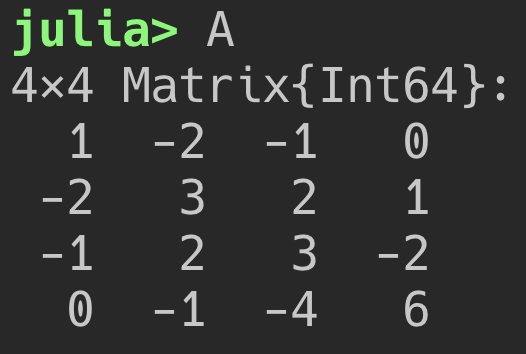
\includegraphics[height=1.5in]{matrix.png}
		            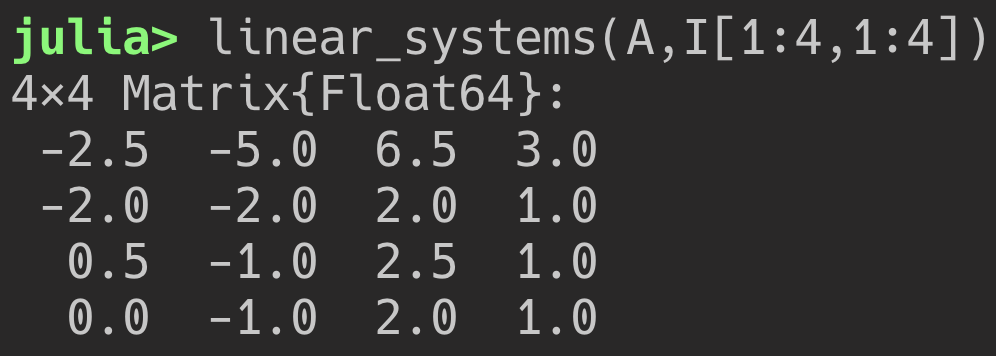
\includegraphics[height=1.5in]{inverse.png}
	      \end{enumerate}

	\item (Julia) Consider the polynomial
	      \[p(x) = (x-2)^9 = x^9 - 18x^8 + 144x^7 - 672x^6 + 2016x^5 - 4032x^4 + 5376x^3 - 4608x^2 + 2304x -512.\]
	      \begin{enumerate}
		      \item Plot \(p(x)\)  for \verb!x = [1.93:0.005:2.07]! using the expanded monomial formula given above. \n\\
		            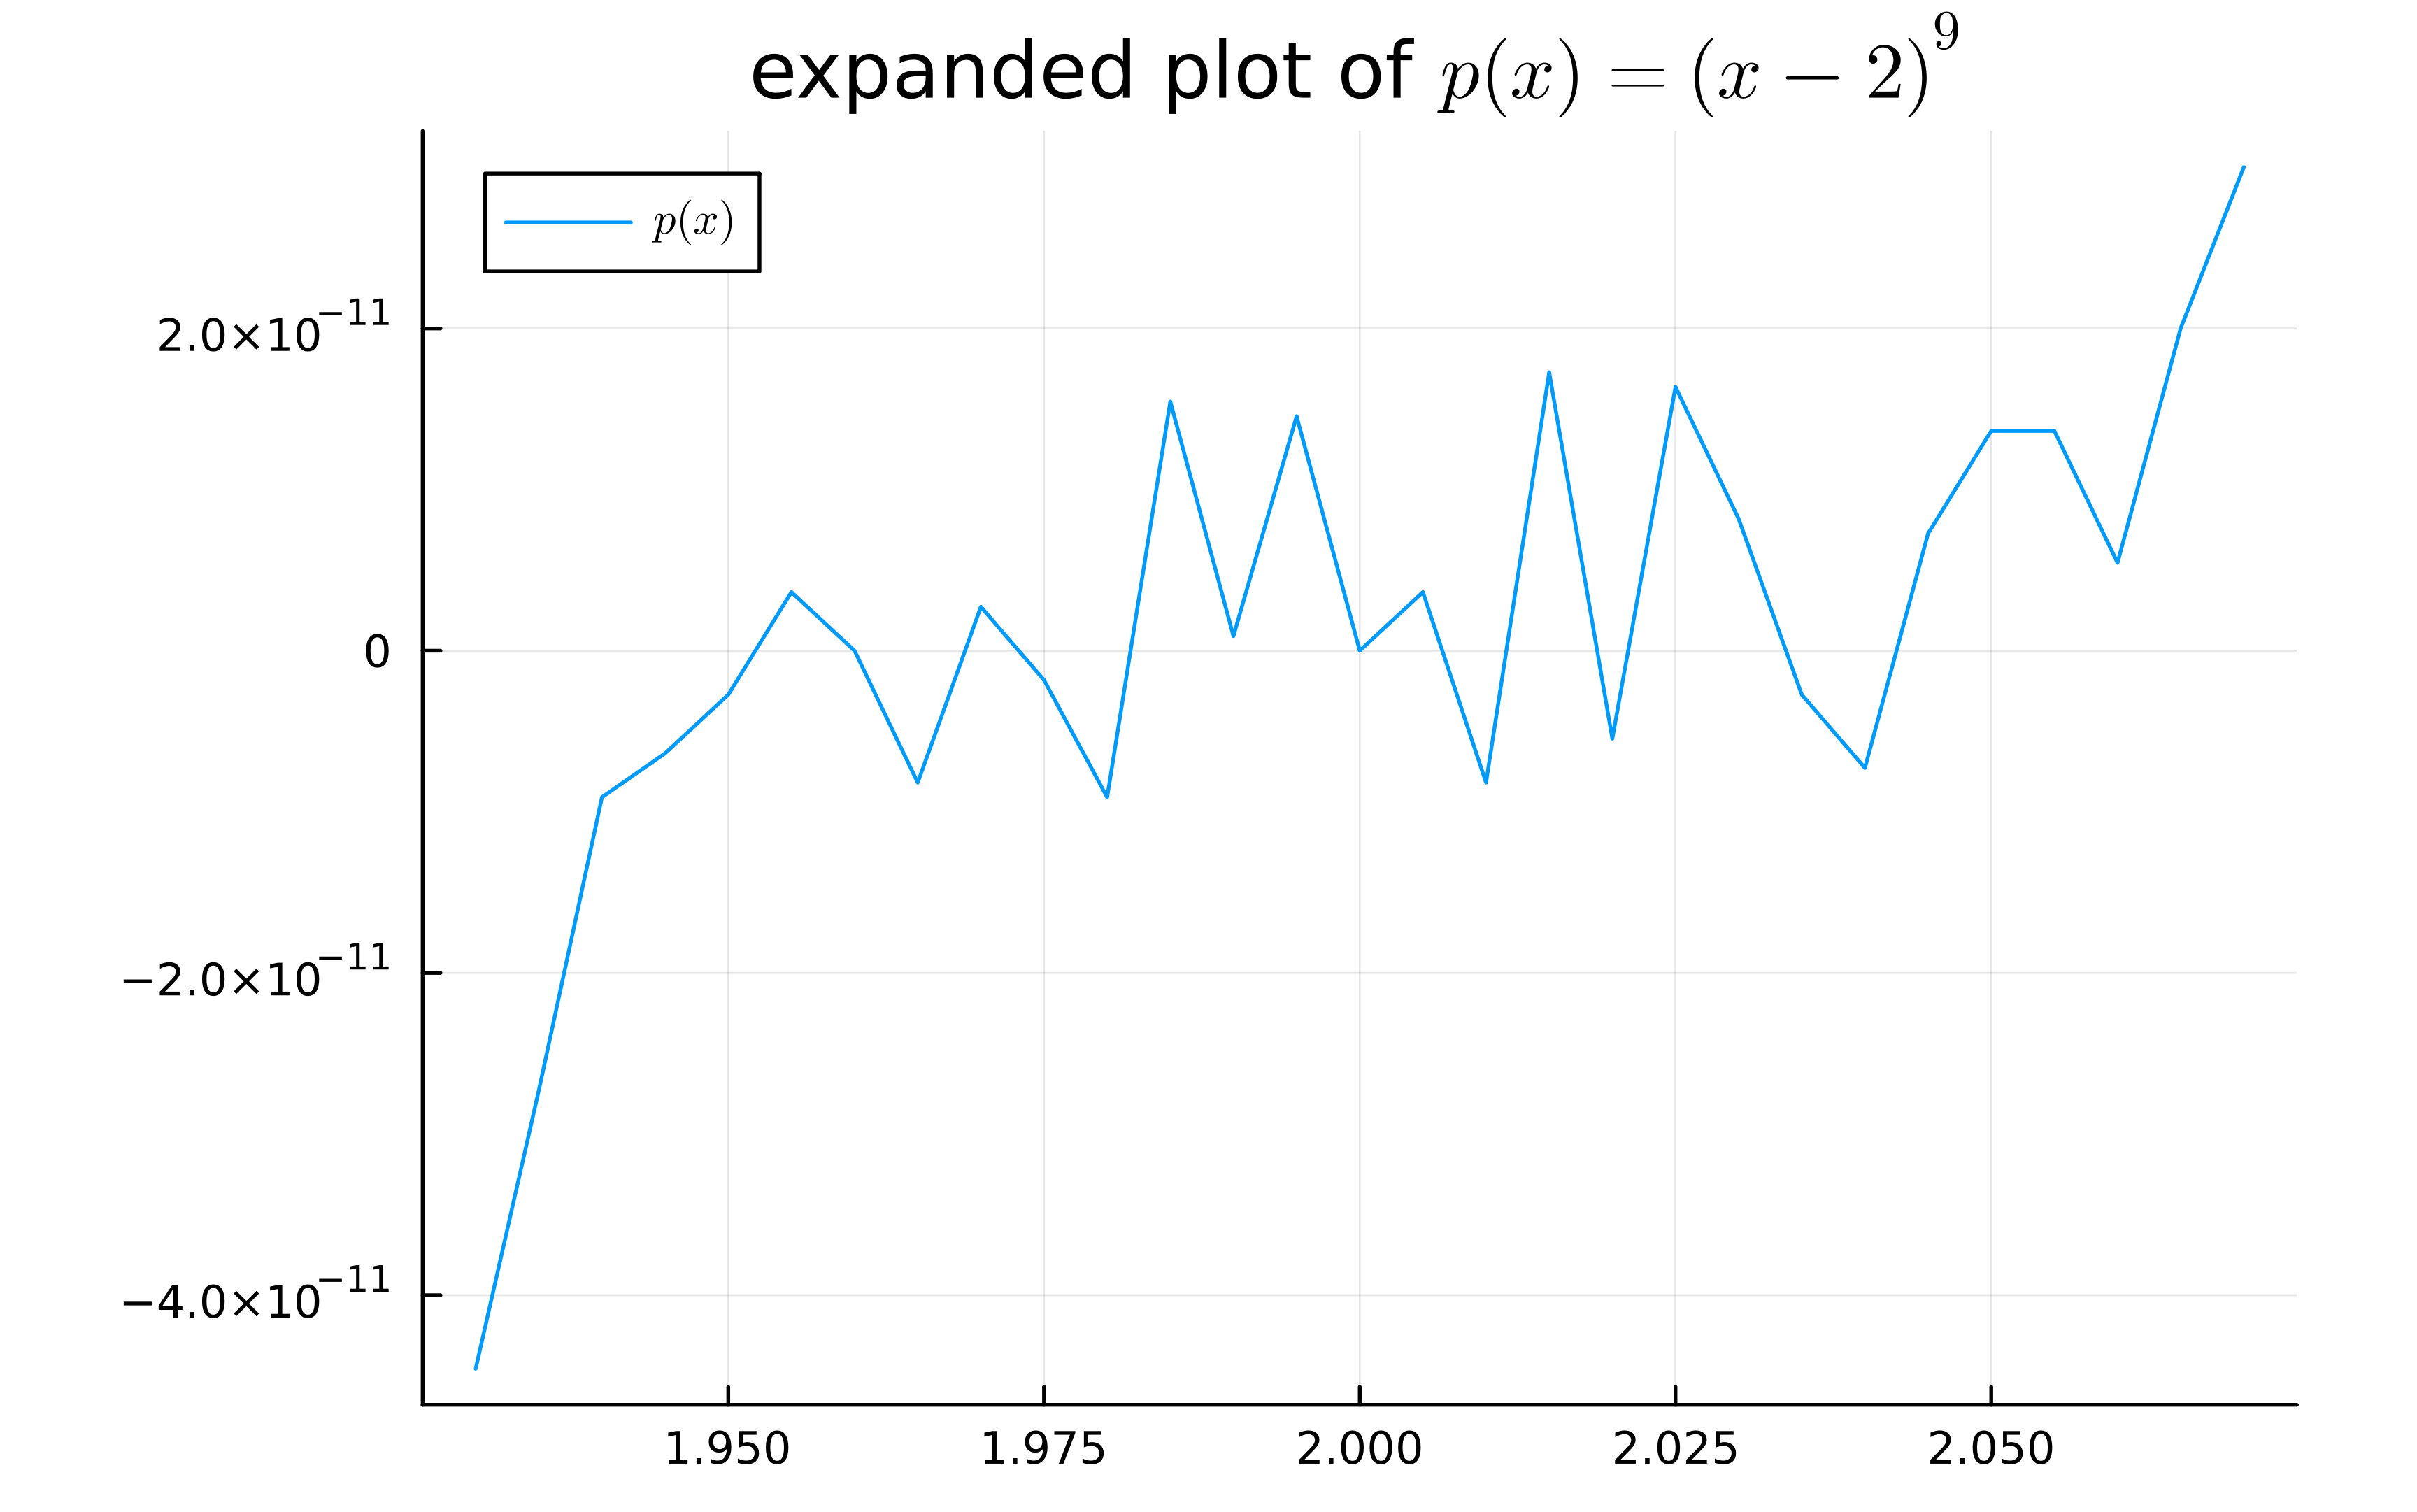
\includegraphics[width=0.8\textwidth]{expanded.png}

		      \item On the same figure, produce another plot of \(p(x)\) with the same points, but now using the original expression \((x-2)^9\). \n\\
		            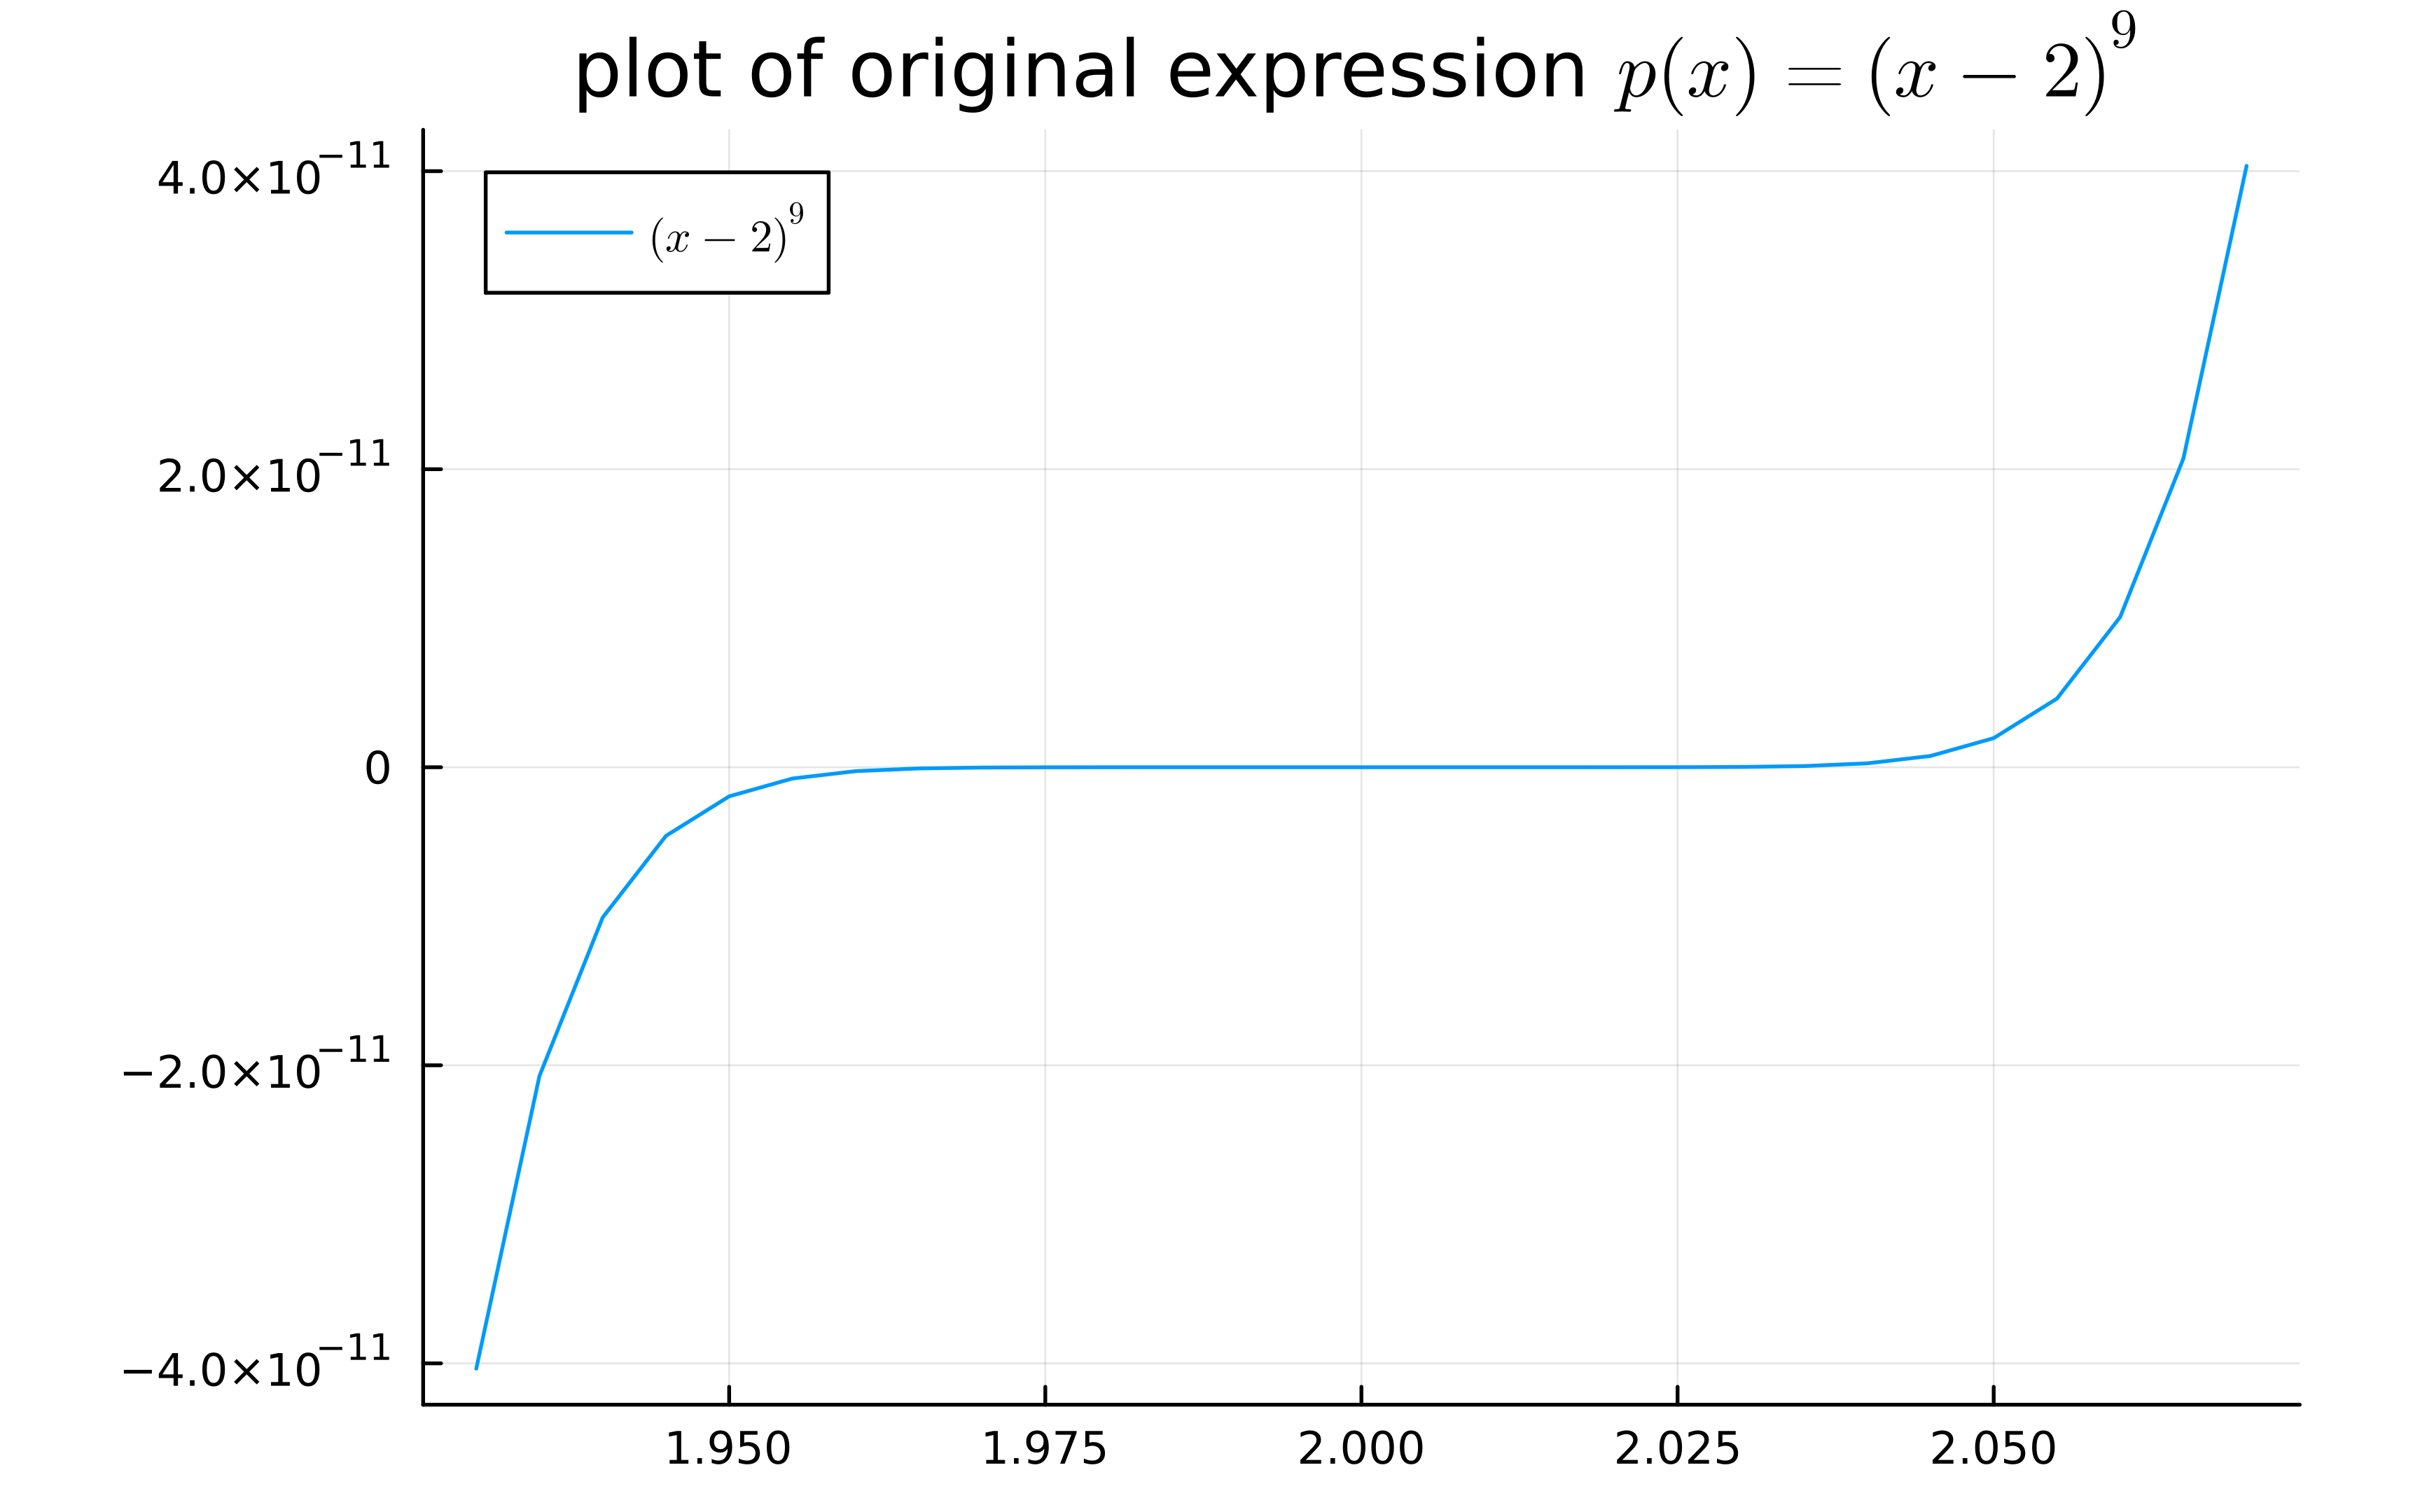
\includegraphics[width=0.8\textwidth]{original.png}

		      \item Coment on what you observe.  Specifically why is one of the methods much less accurate than the other? \n\\
		            idk but I think it could have something to do with the number of operations computed.  If we treat addition and multiplication as one operation (exponentiation counts as 2+ multiplications), then the formula in (a) requires 54 operations for each \(x\), whereas the formula in (b) only requires 9.  More operations means more room for error.
	      \end{enumerate}
\end{enumerate}

\end{document}
